% concatenated from main.tex
\documentclass[conf]{new-aiaa}
%\documentclass[journal]{new-aiaa} for journal papers
\usepackage[utf8]{inputenc}

\usepackage{graphicx}
\usepackage{amsmath}
\let\openbox\relax
\usepackage{amsthm}
\usepackage[version=4]{mhchem}
\usepackage{siunitx}
\usepackage{longtable,tabularx}
\setlength\LTleft{0pt} 
\usepackage{jhoagg}
\usepackage{cleveref}
\usepackage{subcaption}
\usepackage{tikz}
\usetikzlibrary{arrows.meta, shapes.geometric, positioning}


% Use custom style
% \theoremstyle{indentedplain}
\newtheorem{theorem}{Theorem}
\newtheorem{assumption}{Assumption}
\newtheorem{proposition}{Proposition}
\newtheorem{lemma}{Lemma}
\newtheorem{corollary}{Corollary}
\newtheorem{definition}{Definition}
\newtheorem{fact}{Fact}
\newtheorem{conjecture}{Conjecture}
\newtheorem{experiment}{Experiment}
\newtheorem{algorithm3}{Control Design}
\newtheorem{problem}{Problem}

% "Remark" and "Example" to have same look but upright body:
% \theoremstyle{indentedremark}
\newtheorem{remark}{Remark}
\newtheorem{example}{Example}


\allowdisplaybreaks

% Global counters
\newcounter{enumA}
\newcounter{enumC}
\newcounter{enumO}

% (A) enumeration style
\newlist{enumA}{enumerate}{1}
\setlist[enumA,1]{%
  label=(A\arabic*),
  leftmargin=1cm,
  before=\setcounter{enumAi}{\value{enumA}},
  after=\setcounter{enumA}{\value{enumAi}}
}

% (C) enumeration style
\newlist{enumC}{enumerate}{1}
\setlist[enumC,1]{%
  label=(C\arabic*),
  leftmargin=1cm,
  before=\setcounter{enumCi}{\value{enumC}},
  after=\setcounter{enumC}{\value{enumCi}}
}

% (O) enumeration style
\newlist{enumO}{enumerate}{1}
\setlist[enumO,1]{%
  label=(O\arabic*),
  leftmargin=1cm,
  before=\setcounter{enumOi}{\value{enumO}},
  after=\setcounter{enumO}{\value{enumOi}}
}

\title{Geometric Conditions for Lossless Convexification in Linear Optimal Control with Discrete-Valued Inputs: Real-Time Implementation for Spacecraft Rendezvous}

\author{Felipe Arenas-Uribe\footnote{Graduate Research Assistant, Mechanical and Aerospace Engineering, AIAA Student Member.}, Hasan A. Poonawala\footnote{Assistant Professor, Mechanical and Aerospace Engineering.} and Jesse B. Hoagg\footnote{Professor and Chair, Mechanical and Aerospace Engineering, Associate Fellow AIAA.}}
\affil{University of Kentucky, Lexington, Kentucky, 40506}

\begin{document}

\maketitle

\begin{abstract}
    Optimal control problems with discrete-valued inputs are inherently challenging due to their mixed-integer nature, rendering them generally intractable for real-time, safety-critical aerospace applications. Lossless convexification offers a powerful alternative by reformulating these mixed-integer programs into computationally efficient convex programs. This paper develops a lossless convexification framework for the optimal control of linear time-varying systems with discrete-valued inputs. We extend existing theoretical results by demonstrating that system normality is preserved when reformulating Lagrange-form problems into Mayer-form via an epigraph transformation. Furthermore, we establish that under simple geometric conditions on the input set, the solution to the relaxed convex problem strictly satisfies the original non-convex input constraints. This framework enables the real-time computation of optimal discrete-valued controls without resorting to mixed-integer optimization. The proposed algorithm is validated on a spacecraft rendezvous maneuver utilizing discrete-valued reaction thrusters in an elliptical orbit. Numerical results from Monte Carlo simulations confirm that the algorithm consistently yields exact discrete-valued control inputs with computational timelines compatible with safety-critical, on-board applications.
\end{abstract}

\section{Introduction}

Discrete-valued inputs are common in physical systems, as many actuators operate in an on–off manner or with finitely many magnitude levels. Spacecraft performing proximity maneuvers such as rendezvous and capture have actuator configurations that predominantly rely on discrete-valued actuators such as reaction control thrusters \cite{pasand_study_2017}. Optimal control of such systems is computationally challenging since the discrete actuator behavior introduces mixed-integer constraints. Mixed-Integer Programs (MIPs) can numerically solve such control problems, but are inherently difficult to solve, lacking general convergence guarantees and exhibiting exponential growth in runtime with the number of decision variables \cite{junger_mixed_2013}. These computational challenges render MIPs unsuitable for real-time applications such as autonomous vehicle control \cite{malyuta_advances_2021}.

Recent work has used learning-based methods to warm-start MIP solvers and thereby accelerate their convergence \cite{cauligi_coco_2022, cauligi_learning_2020}, by using neural networks in order to provide an initial sub-optimal solution from which the optimizers find an optimal solution. Nonetheless, these strategies provide no formal guarantees of optimality or convergence and need a pre-computed dataset of solutions to train the neural network. An alternative to MIP solvers include homotopy methods. Their core idea is to introduce activation funtions and sequentially solve a continuous problem, adjusting the activation parameters such that the solution takes a mixed-integer behaviour \cite{saranathan_relaxed_2018,malyuta_fast_2023,arya_composite_2021}. However, homotopy methods introduce approximations, which result computationally expensive and does not guarantee optimality of the solution. In contrast, lossless convexification methods have shown that certain MIPs can be reformulated as equivalent convex programs (CPs) without loss of optimality, offering a computationally tractable alternative \cite{malyuta_convex_2022}. A lossless convexification for optimal control problems (OCP) in Mayer-form with linear time-invariant (LTI) systems and disconnected input sets was introduced in \cite{harris_optimal_2021}, where system normality and an extreme-point relaxation were exploited to achieve an exact convex reformulation. Similarly, \cite{woodford_geometric_2022} exploited strong observability to obtain a lossless convexification for a similar problem with state constraints. It was proposed in \cite{harris_optimal_2021} that Lagrange-form problems can be reformulated as Mayer-form problems via an epigraph transformation; however, it remains unclear whether system normality is preserved under this transformation. 

Lagrange-form OCPs include the fuel-optimal control problem, where the $L^1$-norm of the control input serves as the cost function since it is proportional to the total control effort \cite{ross_how_2004}. This problem is particularly relevant in spacecraft applications, where mission lifetime is limited by onboard propellant and maneuvers must therefore be fuel-optimal. Standard trajectory generation algorithms for spacecraft rely in quadratic cost functions which don't minimize fuel consumption directly, which reduces the mission lifetime \cite{ross_space_2006}. In addition, many spacecraft employ discrete-valued actuators—such as cold-gas thrusters in reaction control systems \cite{pasand_study_2017,weston_state---art_2025}. Thus, it is essential to develop real-time fuel-optimal control strategies that explicitly account for discrete inputs.

\begin{figure}[t]
\centering
\includegraphics[width=0.6\linewidth]{Figures/framework.pdf}
%\vspace{-0.15 in}
\caption{Lossless convexification enables real-time solution of optimal control problems with discrete-valued inputs by solving a convex program.}
\label{fig:Framework}
\vspace{-0.15 in}
\end{figure}

In this paper, we extend lossless convexification results from \cite{harris_optimal_2021} and show that Lagrange-form OCPs for linear systems with discrete-valued inputs can be reformulated as a Mayer-form MIP while preserving system normality. We demonstrate that the resulting Mayer-form MIP can be solved as a convex program by leveraging system normality and convex hull relaxation of the input set (see \Cref{fig:Framework}), granted that the input set satisfies certain geometric conditions. To bridge theory and practice, we present a finite-dimensional optimization formulation alongside a bisection algorithm designed to identify a feasible time horizon. The proposed framework is validated through numerical experiments on a spacecraft rendezvous maneuver in an elliptical orbit utilizing discrete-valued reaction thrusters. Finally, we evaluate the impact of discretization coarseness on solution discreteness and conduct Monte Carlo simulations across diverse initial conditions, confirming that the algorithm consistently yields exact discrete-valued controls within timelines compatible with real-time, safety-critical applications.

The remainder of this paper is organized as follows. \Cref{sec:ProblemForm} outlines the problem formulation. \Cref{sec:EquivFormulation} presents an equivalent formulation of the problem. \Cref{sec:LosslessConv} presents the corresponding lossless convexification. Numerical simulation results are provided in \Cref{sec:NumericalSim}, and \Cref{sec:Conclusions} concludes with final remarks and directions for future research.

\section{Problem Formulation}\label{sec:ProblemForm}

\subsection{Notation}

Let $\mathbb{N}_{>0}$ be the set of positive natural numbers not including 0. Consider the set $\SA \subset \mathbb{R}^n$. Then, the convex hull of $\SA$ is $\mathrm{conv}(\SA)$, the extreme points of $\SA$ are $\mathrm{ex}(\SA)$, and the boundary of $\SA$ is $\mathrm{bd}(\SA)$. The vector $e_i$ denotes the $i$-th basis vector of $\mathbb R^m$. Let $f:\mathbb{R}^{n} \to \mathbb{R}$, the \emph{epigraph} of $f$ is $\mathrm{epi}(f) \triangleq \{(x,\mu) \in \mathbb{R}^{n+1}: f(x) \leq \mu\}$. The function $f$ is polyhedral convex if $\mathrm{epi}(f)$ is a polyhedral set.

\subsection{Fuel-Optimal Discrete-Valued Control Problem}

Consider the linear time-varying system
%
\begin{equation}\label{eq:linear_system}
    \dot{x}(t) = A(t) x(t) + B(t) u(t),
\end{equation}
%
where $A(t) \in \mathbb{R}^{n \times n}$, $B(t) \in \mathbb{R}^{n \times m}$, the pair $\big(A(t),B(t)\big)$ is controllable for all $t\geq0$, $x(t) \in \mathbb{R}^n$ is the state, $x(0) = x_0 \in \mathbb{R}^n$ is the initial condition, and $u(t) \in \mathcal{U} \subset \mathbb{R}^m$ is the input. The input set $\mathcal{U}$ is a finite disconnected set
%
\begin{equation}\label{eq:input_set}
    \mathcal{U} \triangleq \{u_1, u_2, \ldots, u_{\ell}\},
\end{equation}
%
where $u_i \in \mathbb{R}^m,\; i=1,\ldots,\ell$ and $\ell \in \mathbb{N}_{>0}$. 

Consider the cost-functional $\psi: \mathbb{R}^n \to \mathbb{R}$, where $\psi(u)$ is a polyhedral convex function. Define $\underline{u} \triangleq \min_{u \in \SU} \psi(u)$ and $\bar{u} \triangleq \max_{u \in \SU} \psi(u)$. Let $\mu \in [\underline{u}, \bar{u}]$ be the slack input of the epigraph $\mathrm{epi}(\psi(u)) = \{(u,\mu) \in \mathbb{R}^{m+1}: \psi(u) \leq \mu\}$. And define the set
%
\begin{equation}\label{eq:relaxed_set}
    \tilde{\SU}_e \triangleq \mathrm{conv}(\SU) \times [\underline{u}, \bar{u}] \cap \mathrm{epi}(\psi(u)).
\end{equation}
%
Then, consider the assumption:
%
\begin{enumA}
    \item $\mathrm{ex}(\tilde{\SU}_e) = \{(u,\mu) \in \mathbb{R}^{m+1}: u \in \SU, \mu = \psi(u)\}.$ \label{ass:augmented_set_vertices}
\end{enumA}
%
This assumption implies that the vertices of the set $\tilde{\SU}_e$ are members of the original input set $\SU$. This geometric property is solely characterized by the function $\psi$ and the set $\SU$. This property will be useful in later sections to enable the lossless convexification of an Optimal Control Problem (OCP). The following examples show sets which satisfy \ref{ass:augmented_set_vertices}.

\begin{example}\label{ex:set_example_1}\rm
    Let $\psi(u) = \|u\|_1$ and consider a system whose input channels can be actuated independently but are limited between two discrete values. Let $u_{\max} > 0$ and define the input set
    %
    \begin{equation*}
        \mathcal{U} \triangleq \{-u_{\max},0,u_{\max}\}^m.
    \end{equation*}
    %
    As seen in \Cref{fig:example1_polytope}, \ref{ass:augmented_set_vertices} is satisfied since all vertices of $\tilde{\SU}_e$ are elements of the set $\SU$. This type of actuator set is common in systems with discrete-valued actuators (e.g. valves or reaction thrusters) who operate independently of each other.
\end{example}

\begin{example}\label{ex:set_example_2}\rm
    Consider a system whose input channels are limited by a magnitude $u_{\max}>0$, and the admissible combinations are constrained such that the 1-norm of the input vector does not exceed this bound.
    \begin{equation*}
        \mathcal{U} \triangleq \{0\}\cup\{\pm u_{\max} e_i : i = 1,\ldots,m\}.
    \end{equation*}
    %
    This structure, shown in \Cref{fig:example2_polytope}, satisfies \ref{ass:augmented_set_vertices} since all vertices of $\tilde{\SU}_e$ are elements of the set $\SU$. The input set considered in this example is common in systems where multiple actuators share a limited total control authority, such that at most one actuator can be fully engaged at any given time. This is the case in small satellite reaction control systems which share a singular propellant tank \cite{weston_state---art_2025}.
\end{example}

\begin{figure}[h]
    \centering
    % First Subfigure (Left)
    \begin{subfigure}[b]{0.48\linewidth}
        \centering
        \includegraphics[width=\linewidth]{Figures/polytopes2.pdf}
        \caption{Input set $\SU$ and its augmented set $\tilde{\mathcal{U}}_e$ from \Cref{ex:set_example_1}.}
        \label{fig:example1_polytope}
    \end{subfigure}
    \hfill % Adds horizontal space to push the subfigures to the edges
    % Second Subfigure (Right)
    \begin{subfigure}[b]{0.48\linewidth}
        \centering
        \includegraphics[width=\linewidth]{Figures/polytopes1.pdf}
        \caption{Input set $\SU$ and its augmented set $\tilde{\mathcal{U}}_e$ from \Cref{ex:set_example_2}.}
        \label{fig:example2_polytope}
    \end{subfigure}
    
    \caption{Comparison of the input sets and their augmented counterparts across different examples.}
    \label{fig:combined_polytopes} % Main figure label for referencing both together
\end{figure}

Let $t_f>0$ be the time horizon. The objective is to solve the optimal control problem:
%
\begin{problem}\rm{Lagrange-Form Mixed-Integer Problem}\label{prob:MICP}
    \begin{subequations}
        \begin{align}
            \min \quad & \int_{0}^{t_f} \psi(u(t)) \, dt \label{eq:cost} \\
            \text{subject to} \quad 
            & \dot{x}(t) = A(t) x(t) + B(t) u(t),\\
            & u(t) \in \mathcal{U}, \label{eq:input_constraints} \\
            & x(0) = x_0, \quad x(t_f) = 0. \label{eq:boundary_conditions}
        \end{align}
    \end{subequations}
\end{problem}

The problem formulation presented in \Cref{prob:MICP} offers a general framework capable of capturing a diverse class of optimal control problems, with particular relevance to aerospace systems. By selecting distinct structural forms for the cost functional $\psi(u)$, this optimization template can be tailored to contrasting operational objectives. For instance, setting $\psi(u) = \|u\|_1$ yields a traditional fuel-optimal control formulation, which is central to high-precision spacecraft maneuvers such as satellite proximity operations, docking, and station-keeping. Alternatively, choosing the zero-pseudonorm $\psi(u) = \|u\|_0$ transforms \Cref{prob:MICP} into the maximum hands-off control problem \cite{nagahara_maximum_2016}. This formulation is especially pertinent to scenarios requiring sparse actuator intervention, finding applications in automotive lane-keeping, aerospace trajectory maintenance, and resource-constrained networked control systems (e.g., packetized or wireless control where communication bandwidth must be strictly conserved).

\section{Equivalent Formulation in Mayer-form}\label{sec:EquivFormulation}

To systematically analyze the convexification properties of \Cref{prob:MICP}, we reformulate the original Lagrange-form OCP into an equivalent Mayer-form OCP. By invoking a standard epigraph transformation, we embed the integral cost into the state \cite{boyd_convex_2023}. This structural shift allows us to leverage convexification frameworks in optimal control literature, such as those established in \cite{harris_optimal_2021}. Define the augmented input set
%
\begin{equation*}
    \mathcal{U}_e \triangleq \{(u,\mu) \in \mathbb{R}^{m+1} : u \in \mathcal{U}, \mu \in [0, \bar{u}],\; \psi(u) \leq \mu\}.
\end{equation*}
%
Next, let $x_c(t) \in \BBR$ be the cost state variable which satisfies the dynamics
%
\begin{equation}\label{eq:cost_state_dynamics}
    \dot{x}_c(t) = \mu(t),
\end{equation}
%
with the initial condition $x_c(0) \triangleq 0$. Define $\hat{u} \triangleq \begin{bmatrix} u & \mu \end{bmatrix}$. Then, the cascade of \cref{eq:linear_system} and \cref{eq:cost_state_dynamics} is
%
\begin{equation} \label{eq:augmented_dynamics}
    \dot{\hat{x}}(t) = \hat{A}(t) \hat{x}(t) + \hat{B}(t)\hat{u}(t),
\end{equation}
%
where
%
\begin{equation*}
    \hat{x} \triangleq \begin{bmatrix} x \\ x_c \end{bmatrix}, \quad
    \hat{A}(t) \triangleq \begin{bmatrix}
        A(t) & 0 \\
        0 & 0
    \end{bmatrix}, \quad \hat{B}(t) \triangleq \begin{bmatrix}
        B(t) & 0 \\
        0 & 1
    \end{bmatrix}.
\end{equation*}
%
Then, consider the Mayer-form OCP:
%
\begin{problem}\rm{Mayer-form Mixed-Integer Problem}\label{prob:MICP_Mayer}
    \begin{subequations}
        \begin{align}
            \min \quad & x_c(t_f) \label{eq:TerminalCost}\\
            \text{subject to} \quad 
            & \dot{\hat{x}}(t) = \hat{A}(t) \hat{x}(t) + \hat{B}(t)\hat{u}(t),\\
            & u_c \in {\mathcal{U}}_e, \label{eq:input_cons}\\
            & x(0) = x_0, \quad x(t_f) = 0, \\
            & x_c(0) = 0
        \end{align}
    \end{subequations}
\end{problem}
%

We now study the equivalency of \Cref{prob:MICP_Mayer} with respect to \Cref{prob:MICP} from an optimal control perspective. Define the Hamiltonian of \Cref{prob:MICP}
%
\begin{equation*}
    H_1(t,x,u,p) \triangleq \psi(u(t)) + p(t)^\top \big( A(t)x(t)+B(t)u(t)\big)
\end{equation*}
%
where $p(t) \in \BBR^n$ is the co-state associated with \cref{eq:linear_system} which satisfies
%
\begin{equation}
    \dot p(t) = - \frac{H_1(t,x,u,p)}{\partial x} = -A(t)^\top p(t)
\end{equation}
%
with the initial condition $p(0) = p_0 \in \BBR^n \setminus \{0\}$ given by the transversality condition \cite[Theorem 6.3.5]{berkovitz_nonlinear_2013}. It follows from the necessary conditions of optimal control \cite[Theorem 6.7.1]{berkovitz_nonlinear_2013}, that the optimal control of \Cref{prob:MICP} is 
%
\begin{equation}\label{eq:optimal_control_p1}
    u^*(t) = \arg \min_{u \in \SU} \big[ H_1(t,x,u,p) \big], \quad \forall t \in [0,t_f].
\end{equation}

Next, define the Hamiltonian of \Cref{prob:MICP_Mayer}
%
\begin{equation*}
    H_2(t,\hat x,\hat u,p, p_c) \triangleq p(t)^\top \big( A(t)x(t)+B(t)u(t)\big) + p_c(t) \mu(t)
\end{equation*}
%
where $p_c(t)$ is the co-state associated with the cost state $x_c(t)$. The terminal cost of \Cref{prob:MICP_Mayer} is $x_c(t_f)$, and therefore the transversality condition yields $p_c(t_f)=\frac{\partial x_c(t_f)}{\partial x_c}=1$. Since $\dot p_c(t) = -\partial H_2/\partial x_c = 0$, the co-state $p_c(t)$ is constant over $[0,t_f]$, thus
%
\begin{equation*}
p_c(t) = 1, \qquad \forall t\in[0,t_f].
\end{equation*}

It follows from the necessary conditions of optimal control \cite[Theorem 6.7.1]{berkovitz_nonlinear_2013}, that the optimal control of \Cref{prob:MICP_Mayer} is 
%
\begin{equation}\label{eq:optimal_control_p2}
    \hat u^*(t) = \arg \min_{\hat u \in \SU_e} \big[ H_2(t,\hat x,\hat u,p, p_c) \big], \quad \forall t \in [0,t_f].
\end{equation}

% The following result shows that the optimal control of \Cref{prob:MICP_Mayer} is also the optimal control of \Cref{prob:MICP}. The proof is in \cite[Section 2.4]{berkovitz_nonlinear_2013}.

The following result shows that the optimal control of \Cref{prob:MICP_Mayer} is also the optimal control of \Cref{prob:MICP}.

\begin{lemma}\rm\label{lemma:MICP2mayer}
A control $u^*(t):[0,t_f]\to\mathbb{R}^m$ minimizes \cref{eq:optimal_control_p1} if and only if the pair $\big(u^*(t),\mu^*(t)\big)$, where $\mu^*(t)=\psi(u^*(t))$, minimizes \cref{eq:optimal_control_p2}. 
\end{lemma}

\begin{proof}
    Fix $t\in[0,t_f]$. By definition of the augmented input set $\mathcal{U}_e$, every admissible pair $(u,\mu)\in\mathcal{U}_e$ satisfies
    %
    \begin{equation*}
    \mu \ge \psi(u).
    \end{equation*}
    %
    Then, for all $(u,\mu) \in \SU_e$,
    %
    \begin{equation*}
    p(t)^\top\big(A(t)x(t)+B(t)u(t)\big) + \mu \geq p(t)^\top\big(A(t)x(t)+B(t)u(t)\big) + \psi(u).
    \end{equation*}
    %
    Equality holds if and only if $\mu=\psi(u)$. Which implies that for all $(u,\mu) \in \SU_e$,
    %
    \begin{equation*}
    H_2(t,\hat x,\hat u,p, p_c) \geq H_1(t,x,u,p).
    \end{equation*}
    
    It follows that
    %
    \begin{equation*}
    \min_{(u,\mu)\in\mathcal{U}_e} H_2(t,\hat x,\hat u,p,p_c)
    =
    \min_{u\in\mathcal{U}} H_1(t,x,u,p),
    \end{equation*}
    %
    and the minimizers satisfy $\mu^*=\psi(u^*)$.
    
    Therefore, $u^*(t)$ minimizes \Cref{eq:optimal_control_p1} if and only if the pair $\big(u^*(t),\mu^*(t)\big)$ with $\mu^*(t)=\psi(u^*(t))$ minimizes \Cref{eq:optimal_control_p2}.
\end{proof}

\section{Normality for Lossless Convexification}\label{sec:LosslessConv}

In this section, we develop a lossless convexification of \Cref{prob:MICP_Mayer} which, by \Cref{lemma:MICP2mayer}, is also valid for \Cref{prob:MICP}. Consider the relaxed augmented set $\tilde{\mathcal{U}}_e$ in \cref{eq:relaxed_set}, which relaxes the input constraint \cref{eq:input_cons} by using a convex hull relaxation of the original input set (i.e. $u \in \mathrm{conv}(\mathcal{U})$). The following result shows that by using the set $\tilde{\mathcal{U}}_e$ as the input constraint, we relax the non-convex constraint \cref{eq:input_cons} to a convex constraint.

\begin{fact}\label{fact:augmented_set_polytope}
The set $\tilde{\mathcal{U}}_e$ is a polytope
\end{fact}

\begin{proof}
Recall that a set is a polytope if it is a bounded polyhedron. We show $\tilde{\mathcal{U}}_e$ is a polyhedron by expressing it as the intersection of finite half-spaces.

Note that the set $\mathrm{conv}(\SU)$ is the convex hull of a finite set of points, thus it is a polytope \cite[Theorem 18.5]{rockafellar_convex_2015}. Since the set $\mathrm{conv}(\SU)$ is a polytope, it follows that it can be represented as the intersection of finite half-spaces \cite[Theorem 1.1]{ziegler_lectures_2007}.

Next, note that the slack input $\mu \in [\underline{u}, \bar{u}]$ is bounded by a pair of linear inequalities $0 \leq \mu \leq \bar{u}$.

Finally, since the function $\psi(u)$ is a convex polyhedral function, it follows that  $\mathrm{epi}(\psi(u)) \triangleq \{(u,\mu) \in \BBR^{n+1}: \psi(u) \leq \mu\}$ is a polyhedral convex set \cite[Corollary 19.2.1]{rockafellar_convex_2015}. Thus, $\tilde{\mathcal{U}}_e$ is a polyhedron. Furthermore, since $\mathrm{conv}(\SU)$ is a polytope, then it is bounded and since $\mu \in [0, \bar{u}]$ is also bounded, then $\tilde{\mathcal{U}}_e$ is bounded making it a polytope.
\end{proof}

Since the set $\tilde{\mathcal{U}}_e$ is a polytope, then we can use its half-space representation to enforce the input constraints as linear constraints. Then, consider the convex relaxation of \Cref{prob:MICP_Mayer}:
%
\begin{problem}\rm{Mayer-form Convex Problem}\label{prob:CP_Mayer}
    \begin{subequations}
        \begin{align}
            \min \quad & x_c(t_f)\\
            \text{subject to} \quad 
            & \dot{\hat{x}}(t) = \hat{A}(t) \hat{x}(t) + \hat{B}(t) \hat{u}(t), \label{eq:Prob_Aug_Dynamics}\\
            & \hat{u} \in \tilde{\mathcal{U}}_e,\\
            & x(0) = x_0, \quad x(t_f) = x_f, \\
            & x_c(0) = 0
        \end{align}
    \end{subequations}
\end{problem}
%
It follows from the necessary conditions of optimal control \cite[Theorem 6.7.1]{berkovitz_nonlinear_2013} the optimal control of \Cref{prob:CP_Mayer} is 
%
\begin{equation}\label{eq:optimal_control_p3}
    \hat u^*(t) = \arg \min_{\hat u \in \tilde{\SU}_e} \big[ H_2(t,\hat x,\hat u,p, p_c) \big], \quad \forall t \in [0,t_f].
\end{equation}

If the minimizer of \cref{eq:optimal_control_p3} over $\tilde{\mathcal{U}}_e$ is not unique, then \cref{eq:optimal_control_p3} does not determine a well-defined control law. To exclude this degeneracy, the concept of normality is defined \cite[Definition 6.7.11]{berkovitz_nonlinear_2013}.

\begin{definition}\rm \label{def:normality}
    The system $(\hat{A},\hat{B})$ is \emph{strongly normal} with respect to $\tilde{\mathcal{U}}_e$ if, for every $p_0 \in \BBR^{n+1} \setminus \{0\}$ and for all but a finite set of points $t \in [0,t_f]$, \eqref{eq:optimal_control_p3} has a unique solution $\hat{u}^*(t) \in \tilde{\mathcal{U}}_e$.
\end{definition}

A fundamental result of normality for linear systems with polytopic input sets is presented next \cite[Corollary 6.7.7]{berkovitz_nonlinear_2013}.

\begin{lemma}\label{lemma:vertices_normality}
    Let $(\hat{A},\hat{B})$ be strongly normal with respect to $\tilde{\mathcal{U}}_e$. Let $\hat{u}^*(t)$ be the unique solution of \eqref{eq:optimal_control_p3} on $[0,t_f]$. Then, $\hat{u}^*(t)$ is piecewise constant on $[0,t_f]$ and for all $t \in [0,t_f]$, $\hat{u}^*(t) \in \mathrm{ex}(\tilde{\mathcal{U}}_e)$.
\end{lemma}

This result implies that the optimal control $\hat{u}^*$ can only take values from a finite set given by the vertices of the input polytope $\tilde{\mathcal{U}}_e$. The next result studies normality of the original system and the augmented system through the epigraph transformation.

\begin{lemma}\rm{ \label{lemma:Normality_augmented}}
    $(A, B)$ is strongly normal with respect to $\mathrm{conv}(\SU)$ if and only if $(\hat{A}, \hat{B})$ is strongly normal with respect to $\tilde{\mathcal{U}}_e$.
\end{lemma}

\begin{proof}
    To prove sufficiency, suppose that $(A,B)$ is strongly normal with respect to $\mathrm{conv}(\SU)$. Then for every $p_0\in\BBR^n\setminus\{0\}$ and for almost every $t$,
    %
    \begin{equation*}
        u^*(t) = \arg \min_{u \in \mathrm{conv}(\SU)} \big[ p(t)^\top\big(A(t)x(t)+B(t)u(t)\big) + \psi(u) \big],
    \end{equation*}
    %
    has a unique solution.
    
    Next, consider the point-wise condition
    %
    \begin{equation*}
        \hat u^*(t) = \arg \min_{\hat u \in \tilde{\mathcal{U}}_e} \big[ p(t)^\top \big( A(t)x(t)+B(t)u(t)\big) + \mu(t) \big].
    \end{equation*}

    Then, the minimizer $\hat u^* = (u^*,\mu^*)$ over $\tilde{\mathcal{U}}_e$ is $(u^*,\psi(u^*))$, where $u^*$ is the unique minimizer of $H_1$. Since $u^*$ is unique and $\psi$ is convex, then $\psi(u^*)$ is unique. Which implies that the minimizer $\hat u^* = (u^*,\mu^*)$ has a unique solution. Thus $(\hat A,\hat B)$ is strongly normal with respect to $\tilde{\mathcal{U}}_e$.
    
    Conversely, suppose $(\hat A,\hat B)$ is normal with respect to $\tilde{\mathcal{U}}_e$. Then for every $p_0\in\BBR^n\setminus\{0\}$ and for almost every $t$,
    %
    \begin{equation*}
        \hat u^*(t) = \arg \min_{\hat u \in \tilde{\mathcal{U}}_e} \big[ p(t)^\top \big( A(t)x(t)+B(t)u(t)\big) + \mu(t) \big].
    \end{equation*}
    %
    has a unique solution. Let $p_0\in\BBR^n\setminus\{0\}$ and it follows from \Cref{lemma:MICP2mayer} that $\hat u^* = (u^*,\mu^*)$, where $\mu^* = \psi(u^*)$. Thus, the point-wise optimality condition is now
    %
    \begin{equation*}
        u^*(t) = \arg \min_{u \in \mathrm{conv}(\SU)} \big[ p(t)^\top \big( A(t)x(t)+B(t)u(t)\big) + \psi(u(t)) \big].
    \end{equation*}
    %
    Which implies that, $(A,B)$ is strongly normal with respect to $\mathrm{conv}(\SU)$.
\end{proof}

This result is useful since it allows for the study of the normality of the augmented system \cref{eq:augmented_dynamics} with respect to $\tilde{\SU}_e$ based on the lower-dimensional system \cref{eq:linear_system} and the set $\mathrm{conv}(\SU)$. Note that the relaxed input set $\mathrm{conv}(\SU)$ can be easily computed offline using a convex hull algorithm, such as the Double Description method \cite{fukuda_double_1996}. Although this algorithm exhibits super-polynomial complexity in the worst case, this does not impede real-time performance, as the half-space representation of the set $\tilde{\SU}_e$ only needs to be computed once offline. The algorithm only requires re-execution if the actuator input set $\mathcal{U}$ is modified.

The next result is the main result, which shows that the optimal control of \Cref{prob:CP_Mayer} is also the optimal control of \Cref{prob:MICP}.

\begin{theorem}\label{thm:CP_for_MICP}
Assume $(A, B)$ is strongly normal with respect to $\mathrm{conv}(\SU)$. Furthermore, assume that \ref{ass:augmented_set_vertices} is satisfied. Let $\big(u^*(t),\mu^*(t)\big)$, where $\mu^*(t)=\psi(u^*(t))$, be the minimizer of \cref{eq:optimal_control_p3}. Then, $u^*(t):[0,t_f]\to \SU$ is the minimizer of \cref{eq:optimal_control_p1} and is piecewise constant on $[0,t_f]$.
\end{theorem}

\begin{proof}
First, we establish the regularity of the optimal control. By \Cref{lemma:Normality_augmented}, the strong normality of $(A, B)$ implies that the augmented system $(\hat{A}, \hat{B})$ is also strongly normal with respect to $\tilde{\mathcal{U}}_e$. Consequently, the minimizer $\hat{u}^*(t) = (u^*(t), \mu^*(t))$ of \cref{eq:optimal_control_p3} is unique. It then follows from \Cref{lemma:vertices_normality} that $\hat{u}^*(t)$ is piecewise constant on $[0,t_f]$ and takes values in the set of extreme points $\mathrm{ex}(\tilde{\SU}_e)$. In view of \ref{ass:augmented_set_vertices}, this ensures that $u^*(t) \in \SU$ for all $t \in [0, t_f]$.

Next, we relate this result to the original control problem. It follows from \cite[Theorem 1]{harris_optimal_2021}, that $\hat{u}^*$ is the unique minimizer of \cref{eq:optimal_control_p2}. Finally, applying \Cref{lemma:MICP2mayer}, we conclude that $u^*$ is the unique minimizer of the original problem \cref{eq:optimal_control_p1}.
\end{proof}

\Cref{thm:CP_for_MICP} formalizes the equivalence between the relaxed convex program \Cref{prob:CP_Mayer} and the original mixed-integer problem \Cref{prob:MICP}, establishing that this formulation constitutes a \textit{lossless convexification}. By mapping the problem to a standard convex program, the optimization can be solved in polynomial time using deterministic interior-point methods or fast first-order solvers \cite{boyd_convex_2023}. Crucially, because the convexification is lossless, the optimal trajectory inherently respects the original discrete control constraints without requiring any ad-hoc heuristic rounding, post-processing, or risking a suboptimality gap. This guarantees both exactness and algorithmic reliability, unlocking the potential for executing complex mixed-integer optimal control strategies on resource-constrained embedded systems, such as onboard spacecraft guidance.

\section{Numerical Simulations}\label{sec:NumericalSim}

We illustrate the application of this lossless convexification framework through a fuel-optimal problem ($\psi(u) = \|u\|_1$) of a low-Earth orbit (LEO) satellite rendezvous maneuver in an elliptical orbit. Consider a non-cooperative chief spacecraft and a chaser spacecraft with cold-gas thruster actuators in its three orthogonal directions, which are saturated at maximum acceleration $u_{\max} = 0.05 \frac{\rm m}{\rm s^2}$, a constraint typical in small satellites \cite{weston_state---art_2025}. The input set has a structure similar to \cref{ex:set_example_1} and is given by
%
\begin{equation*}
    \mathcal{U} \triangleq \{-u_{\max},0,u_{\max}\}^3.
\end{equation*}
%
The relative motion of a chaser spacecraft with respect to a chief in an elliptic orbit is described by Yamanaka-Ankersen (YA) equations \cite{yamanaka_new_2002}. The relative state is $x(t) \triangleq \begin{bmatrix} r(t)^\top & v(t)^\top \end{bmatrix}^\top$, where $r(t) = \begin{bmatrix} x(t) & y(t) & z(t) \end{bmatrix}^\top$ are the radial, along-track, and cross-track displacements, respectively, and $v \triangleq \dot{r}$. The system matrices in \cref{eq:linear_system} are given by
%
\begin{equation*}
A(t) =
\begin{bmatrix}
0 & 0 & 0 & 1 & 0 & 0 \\
0 & 0 & 0 & 0 & 1 & 0 \\
0 & 0 & 0 & 0 & 0 & 1 \\
\dot{\nu}^2 + \dfrac{2\mu}{r_c^3} & \ddot{\nu} & 0 & 0 & 2\dot{\nu} & 0 \\
-\ddot{\nu} & \dot{\nu}^2 - \dfrac{\mu}{r_c^3} & 0 & -2\dot{\nu} & 0 & 0 \\
0 & 0 & -\dfrac{\mu}{r_c^3} & 0 & 0 & 0
\end{bmatrix},
\qquad
B =
\begin{bmatrix}
0 & 0 & 0 \\
0 & 0 & 0 \\
0 & 0 & 0 \\
1 & 0 & 0 \\
0 & 1 & 0 \\
0 & 0 & 1
\end{bmatrix}.
\end{equation*}
%
Here, $r_c(t)$ is the instantaneous orbital radius of the chief spacecraft and $\nu(t)$ is the true anomaly. For a Keplerian orbit with semimajor axis $a$ and eccentricity $e$, the radius and the angular rate satisfy
\begin{equation*}
    r_c(t) = \frac{a(1-e^2)}{1 + e\cos\nu(t)}, \qquad \dot{\nu}(t) = \frac{h}{r_c(t)^2}, 
    \qquad
    h = \sqrt{\mu a (1-e^2)}.
\end{equation*}

% \begin{equation*}
%     \dot{\nu}(t) = \frac{h}{r_c(t)^2}, 
%     \qquad
%     h = \sqrt{\mu a (1-e^2)}.
% \end{equation*}

\subsection{Algorithm Implementation and Time-Horizon Selection}

To solve \Cref{prob:CP_Mayer} numerically, we discretize the time horizon $[0,t_f]$ into $N$ equal intervals of duration $\Delta t = t_f / N$, defining the discrete time instances $t_k = k \Delta t$ for $k = 0, 1, \dots, N$. Applying a zero-order hold (ZOH) to the control input over each interval and assuming the continuous system matrices are approximately constant over each sampling interval, the discrete-time matrices are given by:
%
\begin{equation*}
    \hat{A}_k = \exp\left(\hat{A}(t_k)\Delta t\right), \quad \hat{B}_k = \left(\int_{0}^{\Delta t} \exp\left(\hat{A}(t_k)\tau\right)\mathrm{d}\tau\right)\hat{B}(t_k),
\end{equation*}
%
where $\hat{x}_k = [x_k^T, x_{c,k}]^T$ and $\hat{u}_k$ denote the augmented state and control vectors at the $k$-th sampling node, respectively. This reformulation results in the following optimization problem:
%
\begin{problem}\rm{Discrete-time Mayer-form Convex Problem}\label{prob:CP_Mayer_discrete}
    \begin{subequations}
        \begin{align}
            \min \quad & x_{c,N} \label{eq:Discrete_Objective}\\
            \text{subject to} \quad 
            & \hat{x}_{k+1} = \hat{A}_k \hat{x}_k + \hat{B}_k \hat{u}_k, \quad k = 0, \dots, N-1, \label{eq:Prob_Discrete_Dynamics}\\
            & \hat{u}_k \in \tilde{\mathcal{U}}_e, \quad k = 0, \dots, N-1, \label{eq:Prob_Discrete_Control}\\
            & x_0 = x_0, \quad x_N = x_f, \label{eq:Prob_Discrete_BC}\\
            & x_{c,0} = 0 \label{eq:Prob_Discrete_Cost_Init}
        \end{align}
    \end{subequations}
\end{problem}

This discrete finite-dimensional problem is solved using CVXPY~\cite{diamond_cvxpy_2016} with the ECOS solver on a MacBook Air equipped with an Apple M1 chip and 16~GB of RAM.\footnote{The implementation is available at: \url{https://github.com/FelipeArenasUribe/MICP_LosslessConvexification}}

It is worth noting that in order to solve \Cref{prob:CP_Mayer_discrete}, one must provide a time horizon $t_f$ that allows the optimization problem to be feasible. Selecting an inappropriate $t_f$ can result in an infeasible optimization problem if the horizon is too short to satisfy the boundary conditions under the control bounds, or a sub-optimal trajectory if $t_f$ is unnecessarily long. To solve this challenge, \Cref{prob:CP_Mayer_discrete} can be embedded within a one-dimensional outer-loop optimization algorithm. Let $0<\underline{t}_f < \bar{t}_f<\infty$ be user-defined time limits and consider the time-horizon interval $[\underline{t}_f, \bar{t}_f]$. To find a feasible time-horizon $t^*_f \in [\underline{t}_f, \bar{t}_f]$, a bisection method can be utilized over the interval to locate the smallest $t_f$ for which \Cref{prob:CP_Mayer_discrete} returns a feasible solution. 

As illustrated in \Cref{fig:bisection}, the algorithm initializes the dynamic iteration bounds as $t_\ell = \underline{t}_f$ and $t_u = \bar{t}_f$. At each iteration, the optimization problem is solved using the midpoint horizon $t_{\mathrm{mid}} = (t_\ell + t_u)/2$. If the problem is feasible, the upper bound is updated ($t_u \leftarrow t_{\mathrm{mid}}$); otherwise, the lower bound is updated ($t_\ell \leftarrow t_{\mathrm{mid}}$). This process repeats until the interval narrows below a user-defined convergence tolerance ($t_u - t_\ell \leq \varepsilon$), yielding the optimal feasible horizon $t_f^*$.

\begin{figure}[ht]
\centering
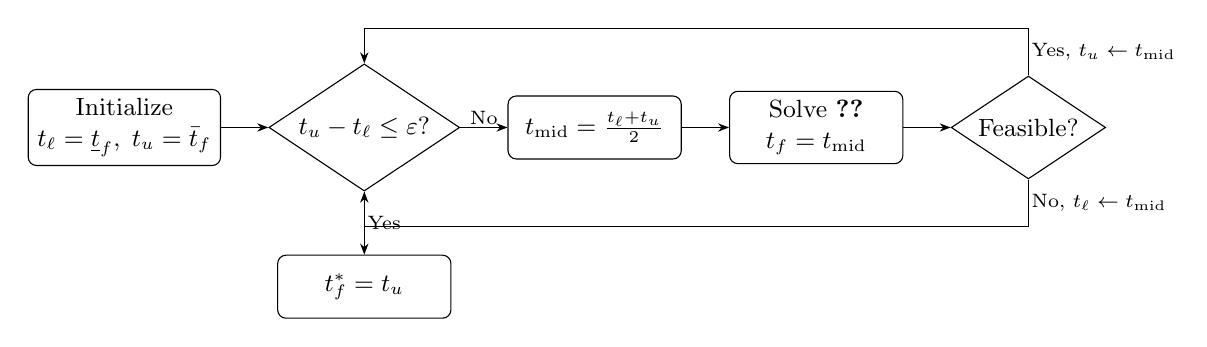
\begin{tikzpicture}[
    node distance = 5mm and 6mm, % Reduced from 6mm and 10mm
    box/.style     = {rectangle, rounded corners=3pt, draw, minimum width=22mm, % Narrowed width
                      minimum height=8mm, align=center, font=\small}, % Lowered height
    decision/.style= {diamond, draw, aspect=1.5, align=center, font=\small,
                      inner sep=2pt},
    arr/.style     = {-{Stealth[length=4pt]}, thin},
    labl/.style    = {font=\scriptsize, inner sep=1pt},
]

%% Nodes (left to right)
\node[box] (init)
    {Initialize\\$t_\ell = \underline{t}_f,\; t_u = \bar{t}_f$};

\node[decision, right=of init] (conv)
    {$t_u - t_\ell \leq \varepsilon$?}; % Combined onto one line to save height

\node[box, right=of conv] (mid)
    {$t_{\mathrm{mid}} = \tfrac{t_\ell+t_u}{2}$};

\node[box, right=of mid] (solve)
    {Solve \Cref{prob:CP_Mayer_discrete}\\$t_f = t_{\mathrm{mid}}$};

\node[decision, right=of solve] (feas)
    {Feasible?};

%% Convergence: YES now exits downward/sideways to keep the profile low
\node[box, below=8mm of conv] (done)
    {$t_f^{\ast} = t_u$};

%% Main flow arrows
\draw[arr] (init)  -- (conv);
\draw[arr] (conv)  -- node[labl,above]{No}  (mid);
\draw[arr] (mid)   -- (solve);
\draw[arr] (solve) -- (feas);

%% Converged: exit downward (saves massive vertical headspace)
\draw[arr] (conv) -- node[labl,right]{Yes} (done);

%% Feasible → tighten upper bound → loop back (Reduced overshoot to 6mm)
\draw[arr] (feas.north) -- ++(0, 6mm)
    node[labl,right,pos=0.5]{Yes, $t_u \leftarrow t_{\mathrm{mid}}$}
    -| (conv.north);

%% Infeasible → raise lower bound → loop back (Reduced overshoot to 6mm)
\draw[arr] (feas.south) -- ++(0,-6mm)
    node[labl,right,pos=0.5]{No, $t_\ell \leftarrow t_{\mathrm{mid}}$}
    -| (conv.south);

\end{tikzpicture}
\caption{Outer bisection loop for time horizon selection.}
\label{fig:bisection}
\end{figure}

The output of \Cref{prob:CP_Mayer_discrete} is a control sequence $\{u_k\}_{k=0}^N$. To evaluate the quality of the solutions, we introduce the following metrics: distance of the input $u_k$ to the discrete set and the average distance of the control sequence to the discrete set, which are defined as
%
\begin{equation*}
    d(u_k) \triangleq \min_{\zeta \in \SU} \| u_k - \zeta \|_2, \quad 
    \bar{d}(u) \triangleq \frac{1}{N} \sum_{k=0}^N \frac{d(u_k)}{u_{\max}}.
\end{equation*}
%
These metrics characterize the discreteness of the solution. Lower values in both metrics imply the control trajectory is closer to satisfying the input constraint $u \in \SU$.

\subsection{Validation of Lossless Convexification}\label{subsec:validation}

We first demonstrate that the the resulting optimal control from the approximation used to solve \Cref{prob:CP_Mayer} is discrete-valued. A discretization grid of $N=1000$ is employed to closely approximate the continuous-time solution. For real-time applications, coarser grids may be adopted to reduce computational effort, as discussed in \cref{subsec:preserving_disc}. 

Consider a chief spacecraft in an elliptical orbit with an eccentricity of $e=0.7$ and a semimajor axis of $a=7102.8 \times 10^3 \text{ m}$. The initial conditions are $r_0 = \begin{bmatrix} -100 & -500 & -100\end{bmatrix}\,\text{m}$ and $v_0 = \begin{bmatrix} 0 & 0 & 0 \end{bmatrix}\,\text{m/s}$. The time horizon is $t_f = 192.1875\,\text{ s}$ which was determined using the bisection algorithm from \Cref{fig:bisection} with $\bar{t}_f = 500.0\,\text{ s}$, $\underline{t}_f=100.0\,\text{ s}$ and $\varepsilon=1.0\,\text{ s}$. The optimization is solved in 0.9782 seconds. \Cref{fig:RendezvousStates} shows the solution of the system's states. Moreover, \Cref{fig:Rendezvoustrajectory} displays the in-plane trajectory of the spacecraft in the Hill frame.

\begin{figure}[ht]
    \centering
    % First Subfigure (Left)
    \begin{subfigure}[b]{0.48\linewidth}
        \centering
        \includegraphics[width=\linewidth]{Figures/rendezvous_example/spacecraft_states_cp.pdf}
        \caption{System states during rendezvous, showing convergence to the desired terminal conditions.}
        \label{fig:RendezvousStates}
    \end{subfigure}
    \hfill % Pushes the subfigures to the left and right edges
    % Second Subfigure (Right)
    \begin{subfigure}[b]{0.48\linewidth}
        \centering
        \includegraphics[width=\linewidth]{Figures/rendezvous_example/ya_trajectory_2d.pdf}
        \caption{Trajectory of fuel-optimal rendezvous maneuver in the radial and along-track plane.}
        \label{fig:Rendezvoustrajectory}
    \end{subfigure}
    
    \caption{Spacecraft states and relative 2D trajectory during the fuel-optimal rendezvous maneuver.}
    \label{fig:RendezvousCombined} % Main label for the entire group
\end{figure}

The optimal control inputs are shown in \Cref{fig:RendezvousInputs}. The dashed lines denote the admissible control values in the discrete set $\SU$. It can be seen that for all $t \in [0,t_f]$, the optimal control satisfies the input constraint $u(t) \in \SU$. The average and normalized average distances to the discrete set are ${d}(u) = 0.000107$ and $\bar{d}(u) = 0.002148$, respectively. These low values indicate that the control sequence remains effectively discrete-valued, despite being computed via the finite-dimensional approximation \Cref{prob:CP_Mayer_discrete} of the original OCP \Cref{prob:MICP}.

\begin{figure}[ht]
    \centering
    \includegraphics[width=0.5\linewidth]{Figures/rendezvous_example/control_inputs_cp.pdf}
    %\vspace{-0.25in}
    \caption{Optimal control inputs with respect to the admissible discrete set $\SU$. The dashed lines represent the admissible inputs.}
    \label{fig:RendezvousInputs}
    %\vspace{-0.1 in}
\end{figure}


\subsection{Preservation of Discrete-Valued Controls Under Reduced Grid Resolution}\label{subsec:preserving_disc}

Real-time implementation requires balancing solver execution time with the need for a discrete-valued control. This introduces an inherent trade-off when selecting the number of sampling instances, $N$. While increasing $N$ aligns the finite-dimensional approximation \Cref{prob:CP_Mayer_discrete} more closely with the continuous formulation \Cref{prob:CP_Mayer}, it simultaneously drives up solver time. Conversely, reducing $N$ expedites the solver at the cost of degrading the discrete-valued nature of the control trajectory, thereby weakening its adherence to the input constraint \cref{eq:input_cons}.

To evaluate this trade-off and investigate the framework's viability for real-time applications, we conduct a parametric study analyzing solution discreteness and solver efficiency across a range of grid sizes. For a fixed time horizon $t_f = 200\,\text{s}$, a batch of 10 initial conditions is uniformly sampled from the state space $\SX_0 \triangleq \{x \in \BBR^6 : \|r\|_{\infty} \leq 500, \|v\|_{\infty} \leq 5\}$. For each initial condition, the finite-dimensional approximation \Cref{prob:CP_Mayer_discrete} is solved over a spectrum of grid points, sweeping $N$ from an initial value of $N_0 = 100$ to a final value of $N_f = 1000$ in increments of 100.

The numerical results of the parametric sweep are illustrated in \Cref{fig:Grid_Tradeoff}, which details the mean solver time and the normalized average distance $\bar{d}(u)$ across the evaluated grid sizes. The mean solver time exhibits a strictly linear dependence on the number of grid points $N$, scaling from approximately $0.025\,\text{s}$ at $N=200$ to $0.017\,\text{s}$ at $N=1000$. Conversely, the normalized average distance decays approximately exponentially as grid density increases. This sharp initial decline highlights a region of diminishing returns, where increasing $N$ beyond a certain threshold yields negligible improvements in control discreteness at the expense of continuous computational overhead. Ultimately, the minimal remaining quantization error at these resolutions is small enough to be readily compensated for through low-level feedback control, validating the framework's suitability for real-time applications.

\begin{figure}[ht]
    \centering
    \includegraphics[width=0.5\linewidth]{Figures/rendezvous_example/grid_size_tradeoff_mean.pdf}
    \vspace{-0.1in}
    \caption{Effect of grid size on solver time and control discreteness. Increasing the number of grid points improves adherence to the discrete control set but increases computational time.}
    \label{fig:Grid_Tradeoff}
\end{figure}

\subsection{Real-Time Performance}\label{subsec:performance}

Real-time spacecraft control guidelines from NASA's Safe \& Precise Landing Integrated Capabilities Evolution (SPLICE) project specify an attitude and position guidance update-rate requirement of 3 seconds, with a target goal of 1 second \cite{sostaric_splice_2021}. Although we focus only on position control, this benchmark provides a meaningful reference for evaluating the computational performance of our algorithm. To assess real-time feasibility, we perform a Monte Carlo simulation in which 1000 initial conditions are uniformly sampled from $\SX_0$. For each sampled initial condition, the OCP is solved with a time horizon of $t_f = 400\,\text{s}$ and $N = 400$ grid points based on the results from \cref{subsec:preserving_disc}.

The Monte Carlo simulation demonstrates that the solver time across all evaluated initial conditions remains well below the 1-second threshold (see \Cref{fig:Solvertime_hist}), successfully satisfying the stringent SPLICE target, a subset of the computed trajectories is displayed in \Cref{fig:mc_trajs}. The resulting profile exhibits a typical right-skewed distribution, featuring a mean solver time of $0.083\,\text{s}$ and a median of $0.069\,\text{s}$. This indicates that while a small subset of challenging initial conditions creates a tail extending toward $0.40\,\text{s}$, the vast majority of cases resolve substantially faster than the target requirement. Furthermore, as shown in \Cref{fig:Distance_hist}, the distribution of the normalized average distance to the discrete control set, $\bar{d}(u)$, is narrowly clustered around a mean of approximately $0.0002$. This highly concentrated profile demonstrates that the algorithm consistently and robustly enforces near-discrete control inputs across the entire operational envelope. Overall, these results confirm that the proposed method simultaneously guarantees deterministic real-time performance and strict control discreteness.

\begin{figure}[ht]
    \centering
    % First Subfigure (Left)
    \begin{subfigure}[b]{0.48\linewidth}
        \centering
        \includegraphics[width=\linewidth]{Figures/rendezvous_example/solver_time_hist.pdf}
        \caption{Histogram of solver times. All solver times are below 1\,s, demonstrating real-time feasibility for the selected grid.}
        \label{fig:Solvertime_hist}
    \end{subfigure}
    \hfill % Distributes the subfigures evenly across the text width
    % Second Subfigure (Right)
    \begin{subfigure}[b]{0.48\linewidth}
        \centering
        \includegraphics[width=\linewidth]{Figures/rendezvous_example/hist_avg_dist.pdf}
        \caption{Histogram of the average distance to the discrete set $\bar{d}(u)$. Small mean value demonstrates that the algorithm reliably produces discrete-valued controls.}
        \label{fig:Distance_hist}
    \end{subfigure}
    
    \caption{Monte Carlo simulation results showing distribution of solver execution times and the distance metrics to the discrete control set.}
    \label{fig:MonteCarloHistograms}
\end{figure}

\begin{figure}
    \centering
    \includegraphics[width=0.65\linewidth]{Figures/mc_trajectories_2d.pdf}
    \caption{Subset of 50 trajectories from the 1000 trajectories computed in the Monte Carlo simulation.}
    \label{fig:mc_trajs}
\end{figure}

\section{Conclusions}\label{sec:Conclusions}

This paper expanded the theoretical and practical boundaries of lossless convexification for linear time-varying systems featuring discrete-valued control inputs. By successfully extending the foundations from \cite{harris_optimal_2021}, we demonstrated that a class of Lagrange-form optimal control problems can be systematically reformulated as a Mayer-form mixed-integer program while strictly preserving system normality. This equivalence is anchored by two primary theoretical contributions. First, \Cref{lemma:Normality_augmented} establishes that system normality is fully preserved when transforming between the Lagrange and Mayer formulations. Second, \Cref{thm:CP_for_MICP} proves that the continuous relaxation provides a lossless convexification of \Cref{prob:MICP}, provided that the system pair $(A, B)$ is strongly normal with respect to $\mathrm{conv}(\SU)$ and that \ref{ass:augmented_set_vertices} is satisfied. Crucially, this latter assumption dictates a definitive geometric condition on the input set $\mathcal{U}$ relative to the cost functional $\psi(u)$, ensuring that the vertices of the relaxed convex input set $\tilde{\mathcal{U}}_e$ map directly to elements of the original discrete input set $\mathcal{U}$.

By exploiting these geometric conditions, this formulation allows the inherently combinatorial mixed-integer problem to be solved reliably as a continuous convex program by leveraging an convex relaxation of the input set under specific geometric conditions. To bridge the gap between theoretical guarantees and algorithmic deployment, we introduced a finite-dimensional approximation alongside an iterative bisection algorithm designed to deterministically identify a feasible time horizon.

Extensive numerical simulations demonstrate that the algorithm consistently yields discrete-valued controls while remaining within real-time computational constraints. These results confirm the practical feasibility and robustness of the proposed framework for safety-critical aerospace applications. Future work will focus on incorporating state constraints into the formulation while strictly preserving input discreteness. Furthermore, the computational efficiency demonstrated by this algorithm positions it as an ideal candidate for closed-loop feedback control via a shrinking-horizon Model Predictive Control (MPC) framework. This strategy will effectively transition the open-loop lossless convexification framework into a robust, closed-loop feedback mechanism capable of enforcing strict input discreteness in real-time.

\bibliography{References}

\end{document}
